\documentclass[border = 0.1cm]{standalone}
\usepackage[utf8]{inputenc}

\usepackage{tikz}
\usepackage{amsfonts, amsmath, amssymb}
\usepackage{systeme, mathtools}
\usetikzlibrary{positioning, arrows.meta, quotes}
\usetikzlibrary{shapes,snakes}
\usetikzlibrary{bayesnet}
\tikzset{>=latex}
\tikzstyle{plate caption} = [caption, node distance=0, inner sep=0pt,
below left=5pt and 0pt of #1.south]

\begin{document}
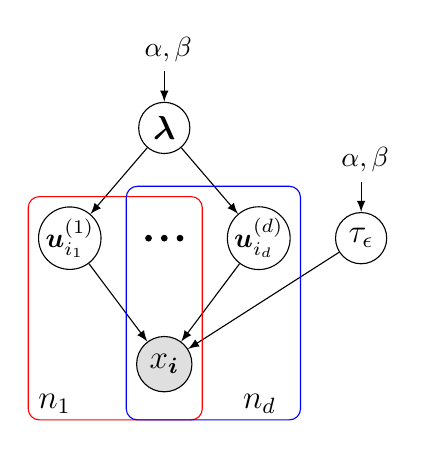
\begin{tikzpicture}
    \node [obs] (x) at (0,0) {\large $x_{\boldsymbol{i}}$};
    \node [circle,draw=black,fill=white,inner sep=0pt,minimum size=0.6cm] (u1) at (-1.2,1.6) { $\boldsymbol{u}_{i_1}^{(1)}$};
    \node [circle,draw=black,fill=white,inner sep=0pt,minimum size=0.6cm] (u3) at (1.2,1.6) { $\boldsymbol{u}_{i_d}^{(d)}$};
    \node [circle,draw=black,fill=white,inner sep=0pt,minimum size=0.65cm] (lambda) at (0,3.0) {\large $\boldsymbol{\lambda}$};

	\node[mark size=1pt,color=black] at (0,1.6) {\pgfuseplotmark{*}};
	\node[mark size=1pt,color=black] at (-0.2,1.6) {\pgfuseplotmark{*}};
	\node[mark size=1pt,color=black] at (0.2,1.6) {\pgfuseplotmark{*}};

    \node [text width=0.5cm] (c0) at (0,4) {$\alpha,\beta$};
    \node [text width=0.5cm] (a0) at (2.5,2.6) {$\alpha,\beta$};
    \node [circle,draw=black,fill=white,inner sep=0pt,minimum size=0.65cm] (tau_epsilon) at (2.5,1.6) {\large $\tau_{\epsilon}$};
    
    \path [draw,->] (u1) edge (x);
    \path [draw,->] (u3) edge (x);
    \path [draw,->] (lambda) edge (u1);
    \path [draw,->] (lambda) edge (u3);

    \path [draw,->] (c0) edge (lambda);
    \path [draw,->] (tau_epsilon) edge (x);
    \path [draw,->] (a0) edge (tau_epsilon);
    \plate [color=red] {part1} {(x)(u1)} { };
    \plate [color=blue] {part3} {(x)(u3)(part1.north east)} { };

    \node [text width=2cm] at (-0.6,-0.5) {\large $n_1$};
    \node [text width=2cm] at (2,-0.5) {\large $n_d$};

\end{tikzpicture}
\end{document}